\chapter{Asking Millionaire Homeowners How They Got Rich}

This lecture begins as a spectacle and only gradually reveals its mechanism. We are shown houses, Ferraris, and nine-figure claims before we are given any clean account of what those numbers mean; then the lecture moves through access, retail economics, tech bootstrapping, portfolio allocation, delegation, sales, creative financing, and finally the limit case in which money ceases to answer the real question. The right way to read the chapter is therefore not as a list of millionaire anecdotes but as a sequence of increasingly explicit models of leverage, with a late correction: wealth can scale a business, but it cannot by itself stabilize a person.

\section{Cold Open: Wealth Before Method}

The opening montage deliberately mixes unlike quantities. A company sale, an annual revenue figure, a projected annual target, and several hype-colored billion claims are all placed side by side. Before we do anything else, we separate the objects.

\begin{table}[h]
\centering
\caption{A bookkeeping ledger for the opening claims}
\begin{tabular}{|l|l|l|}
\hline
Speaker claim & Quantity type & Note \\
\hline
``I sold my last company for \$235 million'' & exit value & relatively clean numerical claim \\
``We did \$850 million for the year'' & annual revenue / sales & operating flow, not exit value \\
``We're going to do a billion this year'' & target annual revenue / sales & projected operating flow \\
``\$235 billion'', ``almost \$100 billion'' & uncertain large-number talk & likely joking, garbled, or inflated \\
\hline
\end{tabular}
\end{table}

A compact notation helps keep the chapter honest:
\begin{align}
S_{\mathrm{exit},1} &= 235\times 10^{6}\ \mathrm{USD},\\
R_{\mathrm{yr},1} &= 850\times 10^{6}\ \mathrm{USD},\\
R_{\mathrm{target},1} &= 10^{9}\ \mathrm{USD}.
\end{align}

The lecture's first question is broad and intentionally unstable: how does somebody become rich now? The early answer is not yet a method of business; it is merely the recognition that wealth appears first as an inaccessible surface.

\section{Boca Raton and the Arithmetic of Access}

The host reframes Miami flash into Boca Raton quiet wealth, and this is the lecture's first serious move. We are no longer asked to stare at wealth; we are asked to get through the gate. The repeated refusals matter structurally because they establish that access is not background noise but the first mechanism in the lecture.

If one cold approach has some success probability \(p_{\mathrm{yes}}\), then after \(n\) approaches the expected number of usable interviews is
\begin{equation}
E[Y_n]=n\,p_{\mathrm{yes}}.
\end{equation}
This is only a schematic reconstruction, but it captures the exact force of the host's line that volume negates luck.

\begin{figure}[h]
\centering
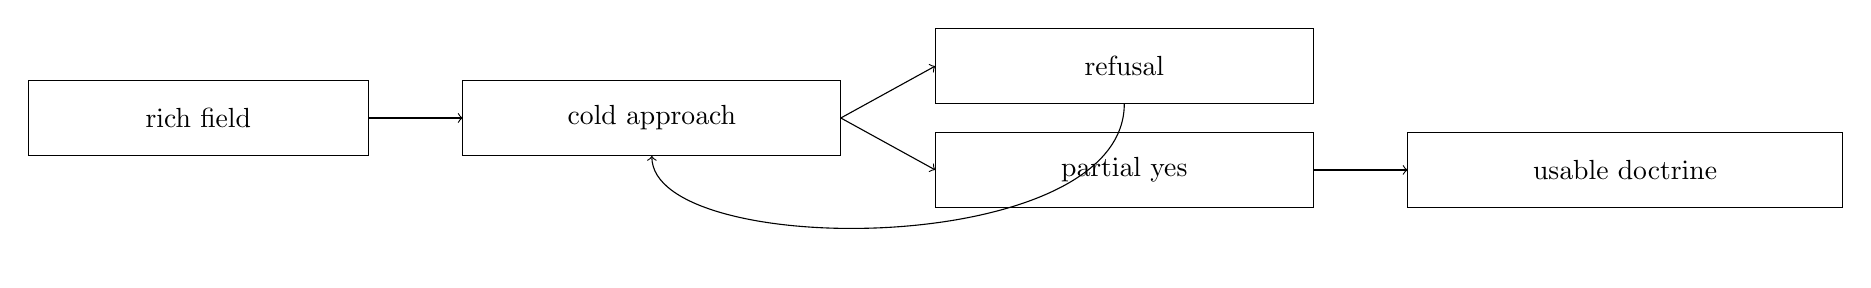
\begin{tikzpicture}[x=2.4cm,y=1.2cm]
\draw (0,0) rectangle (1.8,0.8);
\node at (0.9,0.4) {rich field};

\draw (2.3,0) rectangle (4.3,0.8);
\node at (3.3,0.4) {cold approach};

\draw (4.8,0.55) rectangle (6.8,1.35);
\node at (5.8,0.95) {refusal};

\draw (4.8,-0.55) rectangle (6.8,0.25);
\node at (5.8,-0.15) {partial yes};

\draw (7.3,-0.55) rectangle (9.6,0.25);
\node at (8.45,-0.15) {usable doctrine};

\draw[->] (1.8,0.4) -- (2.3,0.4);
\draw[->] (4.3,0.4) -- (4.8,0.95);
\draw[->] (4.3,0.4) -- (4.8,-0.15);
\draw[->] (6.8,-0.15) -- (7.3,-0.15);
\draw[->] (5.8,0.55) .. controls (5.8,-1.1) and (3.3,-1.1) .. (3.3,0);
\end{tikzpicture}
\caption{A transcript-led access funnel: visibility, refusal, persistence, and occasional extraction of usable knowledge}
\end{figure}

\subsection{Question \& Answer}

\paragraph{Question.} How does access actually work in a field where almost everybody says no?

\paragraph{Answer.} It works by changing the unit of analysis. Instead of treating each refusal as a verdict, the lecture treats each attempt as one trial in a repeated process. Persistence is not ornamental bravado; it is the statistical precondition for obtaining any high-value conversation at all.

\section{From \$10{,}000 to \$100 Million: The E-Cigarette Scale Machine}

The first long interview gives us the lecture's clearest early mechanism. We begin with a small initial capital base, a market with evident defects, and a founder who claims to have worked store to store, mouth to mouth, rather than through abstract growth slogans.

The most concrete arithmetic in the lecture comes from retailer economics. The disposable product is described as selling for \$9.99, with a store cost of \$5.95 and a quoted gross profit of about \(40\%\). Let
\[
P_{\mathrm{retail}}=9.99,\qquad C_{\mathrm{store}}=5.95.
\]
Then the dollar gross profit per unit is
\begin{equation}
G_{\mathrm{store}}=P_{\mathrm{retail}}-C_{\mathrm{store}}=4.04.
\end{equation}
Dividing by the retail price gives
\begin{equation}
m_{\mathrm{store}}=\frac{P_{\mathrm{retail}}-C_{\mathrm{store}}}{P_{\mathrm{retail}}}
=\frac{9.99-5.95}{9.99}\approx 0.4044.
\end{equation}
So the spoken ``40\% GP'' is close to the explicit arithmetic.

The lecture then adds a second layer: simplification. The product was not merely cheaper or more profitable; it was easier to choose. That is why the nicotine ladder and the white-box cigarette labels matter. The founder is reducing cognitive friction at the point of sale.

\begin{table}[h]
\centering
\caption{Simplification at the counter}
\begin{tabular}{|l|l|}
\hline
Customer-facing cigarette label & Logic recommendation \\
\hline
Marlboro & Logic Platinum \\
Marlboro Light & Logic Gold Label \\
Newport & identified but exact paired Logic line not fully specified \\
\hline
\end{tabular}
\end{table}

The nicotine levels are reported only as spoken markers,
\[
N=\{2.7,\,1.8,\,1.5,\,<1\},
\]
and we leave their units unspecified because the transcript does not settle them.

The operational loop can be drawn very simply:
\begin{figure}[h]
\centering
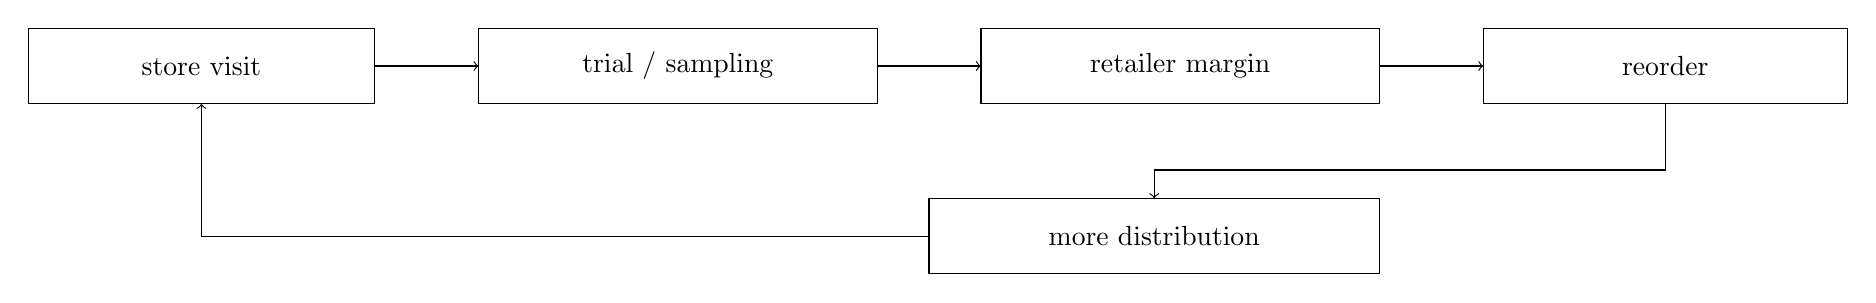
\begin{tikzpicture}[x=2.2cm,y=1.2cm]
\draw (0,0) rectangle (2,0.8);
\node at (1,0.4) {store visit};

\draw (2.6,0) rectangle (4.9,0.8);
\node at (3.75,0.4) {trial / sampling};

\draw (5.5,0) rectangle (7.8,0.8);
\node at (6.65,0.4) {retailer margin};

\draw (8.4,0) rectangle (10.5,0.8);
\node at (9.45,0.4) {reorder};

\draw (5.2,-1.8) rectangle (7.8,-1);
\node at (6.5,-1.4) {more distribution};

\draw[->] (2,0.4) -- (2.6,0.4);
\draw[->] (4.9,0.4) -- (5.5,0.4);
\draw[->] (7.8,0.4) -- (8.4,0.4);
\draw[->] (9.45,0) -- (9.45,-0.7) -- (6.5,-0.7) -- (6.5,-1);
\draw[->] (5.2,-1.4) -- (1,-1.4) -- (1,0);
\end{tikzpicture}
\caption{A scale loop reconstructed from the e-cigarette interview}
\end{figure}

The lecture's quantitative endpoints are then stated in escalating order: a start with \$10{,}000, a biggest year of \$100 million, \(100{,}000\) points of distribution, and breaking \$100 million in \(18\) months before a sale in under five years. Here the transcript is less interested in accounting detail than in one clear thesis: the growth machine is built from repeated local advantages rather than from a single grand insight.

\subsection{Question \& Answer}

\paragraph{Question.} How do we find the real market problem inside a crowded category?

\paragraph{Answer.} The lecture's answer is empirical rather than theoretical. We go into the stores, ask what sells, ask what fails, ask what gets returned, and then design around those frictions. In this case the defect is a combination of product failure, high cost, and too much choice without guidance.

\section{Bootstrapping a Tech Exit: Timing, Sales, and Mentor Multiplication}

The next long case keeps the same initial cash figure but changes the mechanism entirely. The founder starts from a grandmother's \$10{,}000 loan, refuses outside financing, works from a kitchen table, sells to advertisers, and tries to displace billboards and yellow pages. This is not a retail-distribution story. It is a timing-and-demand story, together with a people story.

We can write the bootstrap path in a stripped form:
\begin{align}
K_{\mathrm{boot,tech}} &= 10{,}000\ \mathrm{USD},\\
\text{external raise} &= 0,\\
S_{\mathrm{exit},2} &= 235\times 10^{6}\ \mathrm{USD}.
\end{align}
The lecture then names the attributed drivers without pretending to derive them:
\[
\{\text{innovation},\ \text{market demand},\ \text{timing},\ \text{luck},\ \text{people}\}.
\]

The most useful analytic turn in this section is the shift from ``being good at business'' to finding the right people and the right mentors. The lecture does not give a formula, but it does imply a multiplicative effect: a mentor shortens search, prevents emotional mistakes, and accelerates scaling. One could schematize this as
\begin{equation}
\text{effective learning rate with mentor}>\text{effective learning rate alone},
\end{equation}
but the real content lies in the sequence rather than the notation: first bootstrap, then sell, then negotiate without emotional leakage, then compound by borrowing experienced judgment.

\subsection{Question \& Answer}

\paragraph{Question.} What distinguishes this tech path from the retail path we just saw?

\paragraph{Answer.} The lecture puts the contrast in the causal chain. The e-cigarette story scales through the street, the store, the retailer, and the distribution point; the tech story scales through timing, advertiser demand, negotiation discipline, and the assembly of people the founder herself could not replace by code or capital alone.

\section{Risk After the Exit: Entrepreneurship and Portfolio Choice}

The shorter Ferrari and specialty-finance case widens the lecture from company building to capital deployment. The speaker's advice is simple and severe: do not expect a large company to make you rich; if one wants a very large upside, one must build something for oneself. This is then tied to later-life risk and to an explicit portfolio comparison.

The lecture gives a rule-of-thumb result and then immediately breaks it. The speaker says the old heuristic would put someone in his position at roughly
\begin{equation}
w_{\mathrm{eq}}^{\mathrm{rule}}=35\%,
\end{equation}
but his reported allocation is
\begin{equation}
w_{\mathrm{eq}}^{\mathrm{reported}}=95\%.
\end{equation}
For crypto he offers a moderate-risk suggestion
\begin{equation}
w_{\mathrm{crypto}}^{\mathrm{modest}}\in[10\%,15\%],
\end{equation}
while also saying that his own profile is closer to
\begin{equation}
w_{\mathrm{crypto}}^{\mathrm{self}}=25\%.
\end{equation}
These are speaker-attributed choices, not normative finance theory, and the percentages do not combine neatly enough to be treated as a closed allocation model. Still, the lecture clearly wants us to hear the contrast between rule, conviction, and risk tolerance.

\subsection{Question \& Answer}

\paragraph{Question.} What should risk look like once somebody is already rich?

\paragraph{Answer.} The lecture does not give a universal answer. It gives a pattern: continue to take risk, but do so under an explicit view of the future, and distinguish between the old heuristic, the speaker's own conviction, and the risk profile appropriate for somebody else.

\section{Sean Mike: Need-Based Business, Delegation, and the Presumptive Sale}

The Sean Mike segment is the lecture's central synthesis. By the time we arrive here, the lecture has already shown bootstrap capital, distribution, negotiation, and portfolio choice. Now it shows how a business becomes larger than the founder.

The first thesis is about need-based products. The life-insurance business is called unsexy but profitable precisely because demand does not depend on glamour. The second thesis is that enormous scale requires us to stop identifying the firm with the founder's own hands.

A clean formalization is possible. Normalize solo throughput to one unit:
\[
T_{\mathrm{solo}}=1.
\]
If delegate \(i\) contributes a fraction \(\alpha_i\) of that normalized output, then delegated throughput is
\begin{equation}
T_{\mathrm{delegated}}=\sum_{i=1}^{n}\alpha_i.
\end{equation}
The lecture's practical claim is that scale begins once
\begin{equation}
T_{\mathrm{delegated}}>T_{\mathrm{solo}},
\end{equation}
that is, once the sum of trained, trusted operators exceeds what the founder could do by personal effort alone.

\begin{figure}[h]
\centering
\begin{tikzpicture}[x=2.5cm,y=1.5cm]
\draw (0,0) rectangle (2.2,0.9);
\node at (1.1,0.45) {founder};

\draw (-3,-2) rectangle (-0.8,-1.1);
\node at (-1.9,-1.55) {lead generation};

\draw (-0.2,-2) rectangle (2,-1.1);
\node at (0.9,-1.55) {marketing};

\draw (2.6,-2) rectangle (4.8,-1.1);
\node at (3.7,-1.55) {recruiting};

\draw (5.4,-2) rectangle (7.6,-1.1);
\node at (6.5,-1.55) {tech / ops};

\draw[->] (1.1,0) -- (-1.9,-1.1);
\draw[->] (1.1,0) -- (0.9,-1.1);
\draw[->] (1.1,0) -- (3.7,-1.1);
\draw[->] (1.1,0) -- (6.5,-1.1);
\end{tikzpicture}
\caption{Delegation as a throughput multiplier rather than a founder's loss of control}
\end{figure}

The sales doctrine that follows is equally structured. The lecture rejects generic cold calling in favor of qualified leads, rejects timid asking in favor of presumptive framing, and rejects manipulative charm in favor of plain truth. One useful schematic is
\begin{equation}
C_{\mathrm{sales}}\propto L_{\mathrm{qualified}}\cdot q_{\mathrm{presume}}\cdot q_{\mathrm{truth}},
\end{equation}
where \(L_{\mathrm{qualified}}\) is usable lead volume, \(q_{\mathrm{presume}}\) measures how strongly the salesperson moves the conversation toward action, and \(q_{\mathrm{truth}}\) measures the credibility gained by directness.

\subsection{Question \& Answer}

\paragraph{Question.} How does delegation turn one operator into a billion-dollar machine?

\paragraph{Answer.} By redistributing action without abandoning direction. The lecture insists that if we can teach somebody else to do a task, even at lower individual efficiency, then the aggregate organization can outperform the founder working alone. The deeper point is psychological: scale requires us to tolerate the bad decision, the imperfect rep, and the fall on the face, because otherwise we remain trapped inside our own labor.

\subsection{Question \& Answer}

\paragraph{Question.} What does presumptive selling actually mean?

\paragraph{Answer.} It means that once need is established, the conversation moves as though action is the natural next state. The airport tipping example is the lecture's miniature model: not ``would you like to do anything at all?'' but ``which form will the action take?'' This is then yoked to truth-telling, because the lecture claims that the buyer's main fear is not price but deception.

\section{Real Estate, Drawdown, and the Inner Problem of Wealth}

The final interview begins as a real-estate lesson and ends as a correction to the whole lecture. First we get the fourplex story: live in one unit, rent the other three, reduce out-of-pocket exposure, then move to better structures, better credit, and eventually creative financing. The cash ladder can be written exactly as the speaker gives it:
\begin{align}
K_1 &= 50{,}000\ \mathrm{USD},\\
K_2 &= 5{,}000\ \mathrm{USD},\\
K_3 &= 3{,}000\ \mathrm{USD},\\
V_4 &= 72\times 10^{6}\ \mathrm{USD},\qquad K_4=0.
\end{align}
The lecture does not give the algebra of the zero-money structure, so we do not invent it. We preserve only the mechanism named in speech: reputation, credit, willing capital, and deal-finding.

\subsection{Question \& Answer}

\paragraph{Question.} Do we need a lot of money to start in real estate?

\paragraph{Answer.} Not according to this interview. The lecture's answer is sequential rather than absolute: start with a small structure, let occupancy and rent reduce effective burden, build reputation, then move into transactions whose capital stack no longer resembles the first purchase.

Then the interview turns downward. A year of severe loss is named:
\begin{equation}
L_{\mathrm{yr}}=250\times 10^{6}\ \mathrm{USD}.
\end{equation}
But the speaker immediately says that the important object is not the loss itself. The important object is the habit of external validation, the collapse of identity into business, and the discovery that money buys time rather than happiness.

The lecture's late recovery rule can be rendered, cautiously, as
\begin{equation}
x_{t+1}=1.01\,x_t.
\end{equation}
Here \(x_t\) does not represent wealth. It represents the speaker's idea of recovery by baby steps, one percent at a time, with conversation and self-contact replacing sedative overwork.

\begin{figure}[h]
\centering
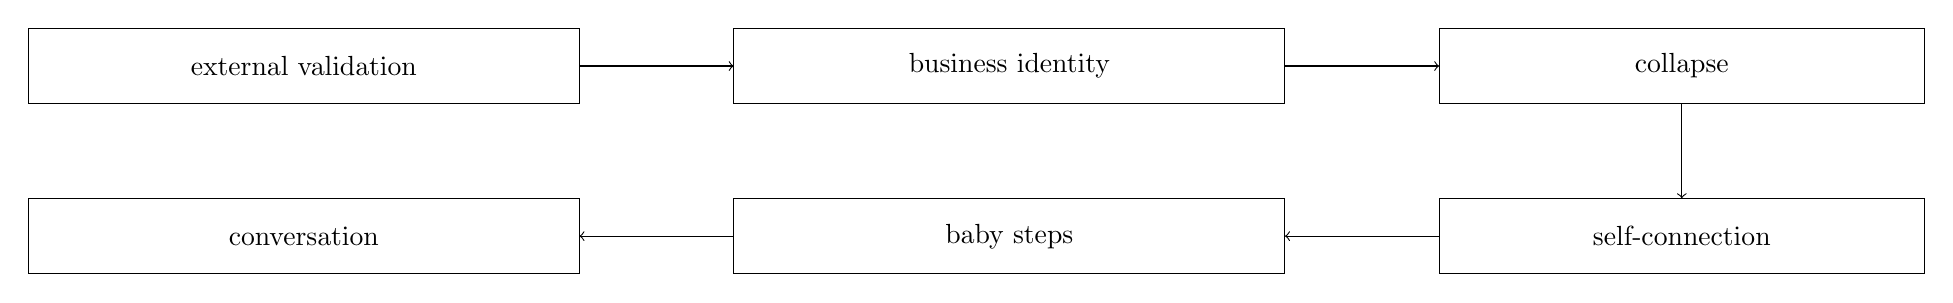
\begin{tikzpicture}[x=2.8cm,y=1.2cm]
\draw (0,0) rectangle (2.5,0.8);
\node at (1.25,0.4) {external validation};

\draw (3.2,0) rectangle (5.7,0.8);
\node at (4.45,0.4) {business identity};

\draw (6.4,0) rectangle (8.6,0.8);
\node at (7.5,0.4) {collapse};

\draw (0,-1.8) rectangle (2.5,-1);
\node at (1.25,-1.4) {conversation};

\draw (3.2,-1.8) rectangle (5.7,-1);
\node at (4.45,-1.4) {baby steps};

\draw (6.4,-1.8) rectangle (8.6,-1);
\node at (7.5,-1.4) {self-connection};

\draw[->] (2.5,0.4) -- (3.2,0.4);
\draw[->] (5.7,0.4) -- (6.4,0.4);
\draw[->] (7.5,0) -- (7.5,-1);
\draw[->] (6.4,-1.4) -- (5.7,-1.4);
\draw[->] (3.2,-1.4) -- (2.5,-1.4);
\end{tikzpicture}
\caption{The late inversion of the lecture: from outer success to inner repair}
\end{figure}

\subsection{Question \& Answer}

\paragraph{Question.} What does money fail to solve?

\paragraph{Answer.} The lecture's final answer is that money solves constraint and buys time, but it does not by itself produce identity, peace, or self-knowledge. If the self has been outsourced to business success, then even very large money can amplify the distortion rather than cure it.

\section{Summary}

The lecture begins by placing us in front of wealth and asking us to stare. It then forces us to separate quantity from quantity, access from display, margin from story, leads from hustle, delegation from control, and capital structure from mere cash. The final correction is the most important one: business scale can be modeled, and much of the chapter has done exactly that, but the lecture refuses to end there. Its last lesson is that a wealth process without a self is unstable, and that the person must eventually become part of the model.